\documentclass[12pt]{beamer}
\usepackage{../Estilos/BeamerMAF}
%Sección para el tema de beamer, con el theme, usercolortheme y sección de footers
\usetheme{CambridgeUS}
\usecolortheme{beaver}
%\useoutertheme{default}
\setbeamercovered{invisible}
% or whatever (possibly just delete it)
\setbeamertemplate{section in toc}[sections numbered]
\setbeamertemplate{subsection in toc}[subsections numbered]
\setbeamertemplate{subsection in toc}{\leavevmode\leftskip=3.2em\rlap{\hskip-2em\inserttocsectionnumber.\inserttocsubsectionnumber}\inserttocsubsection\par}
\setbeamercolor{section in toc}{fg=blue}
\setbeamercolor{subsection in toc}{fg=blue}
\setbeamercolor{frametitle}{fg=blue}
\setbeamertemplate{caption}[numbered]

\setbeamertemplate{footline}
\beamertemplatenavigationsymbolsempty
\setbeamertemplate{headline}{}


\makeatletter
\setbeamercolor{section in foot}{bg=gray!30, fg=black!90!orange}
\setbeamercolor{subsection in foot}{bg=blue!30!yellow, fg=red}
\setbeamercolor{date in foot}{bg=black, fg=white}
\setbeamertemplate{footline}
{
  \leavevmode%
  \hbox{%
  \begin{beamercolorbox}[wd=.333333\paperwidth,ht=2.25ex,dp=1ex,center]{section in foot}%
    \usebeamerfont{section in foot} \insertsection
  \end{beamercolorbox}%
  \begin{beamercolorbox}[wd=.333333\paperwidth,ht=2.25ex,dp=1ex,center]{subsection in foot}%
    \usebeamerfont{subsection in foot}  \insertsubsection
  \end{beamercolorbox}%
  \begin{beamercolorbox}[wd=.333333\paperwidth,ht=2.25ex,dp=1ex,right]{date in head/foot}%
    \usebeamerfont{date in head/foot} \insertshortdate{} \hspace*{2em}
    \insertframenumber{} / \inserttotalframenumber \hspace*{2ex} 
  \end{beamercolorbox}}%
  \vskip0pt%
}
\makeatother\newlength{\depthofsumsign}
\setlength{\depthofsumsign}{\depthof{$\sum$}}
\newcommand{\nsum}[1][1.4]{% only for \displaystyle
    \mathop{%
        \raisebox
            {-#1\depthofsumsign+1\depthofsumsign}
            {\scalebox
                {#1}
                {$\displaystyle\sum$}%
            }
    }
}
\def\scaleint#1{\vcenter{\hbox{\scaleto[3ex]{\displaystyle\int}{#1}}}}
\def\bs{\mkern-12mu}





\date{}
\title{Bases de vectores no ortogonales}
\author{M. en C. Abraham Lima Buendía \\ M. en C. Gustavo Contreras Mayén}

\begin{document}
\maketitle
\fontsize{14}{14}\selectfont
\spanishdecimal{.}

\section*{Contenido}
\frame{\tableofcontents[currentsection, hideallsubsections]}

\section{Introducción}
\frame{\tableofcontents[currentsection, hideothersubsections]}
\subsection{Referencia previa}

\begin{frame}
\frametitle{Lo que ya conocemos}
En cursos previos en la carrera, has conocido el manejo de una base ortonormal canónica para vectores en $\mathbb{R}^{n}$, en esta parte previa del curso, revisamos una alternativa para dichas bases, ya que en diferentes fenómenos físicos una base canónica no siempre es la mejor opción para su modelado.
\end{frame}
\begin{frame}
\frametitle{Nuevos conceptos}
Si bien nos mantendremos en vectores en $\mathbb{R}^{3}$ la revisión de este revisión de este material sentará las bases para la construcción del concepto de \textbf{covarianza}, \textbf{contravarianza}, \textbf{tensor métrico} y \textbf{notación de índices}, mismos que serán extendidos a variedades diferenciables en las primeras semanas del curso.
\end{frame}

\section{Bases no ortogonales}
\frame{\tableofcontents[currentsection, hideothersubsections]}
\subsection{Vectores no ortogonales}

\begin{frame}
\frametitle{Usando vectores}
Consideramos un conjunto de vectores en $\mathbb{R}^{n}$ $\left\{ \va{b}_{1}, \va{b}_{2}, \va{b}_{3}  \right\}$, ahora analizamos las condiciones suficientes y necesarias para poder escribir a un vector $\va{A}$ en términos de estos tres vectores:
\begin{align}
\va{A} = \alpha^{*}_{1} \, \va{b}_{1} + \alpha^{*}_{2} \, \va{b}_{2} + \alpha^{*}_{3} \, \va{b}_{3}
\label{eq:ecuacion_01_01}
\end{align}
\end{frame}
\begin{frame}
\frametitle{Descomposición en la base canónica}
Si se descompone la expresión de la ec. (\ref{eq:ecuacion_01_01}) en la base canónica, implica el desarrollo de las siguientes tres igualdades:
\pause
\begin{align}
\begin{aligned}
A_{x} &= \alpha^{*}_{1} \, \va{b}_{1,x} + \alpha^{*}_{2} \, \va{b}_{2,x} + \alpha^{*}_{3} \, \va{b}_{3,x} \\[0.5em]
A_{y} &= \alpha^{*}_{1} \, \va{b}_{1,y} + \alpha^{*}_{2} \, \va{b}_{2,y} + \alpha^{*}_{3} \, \va{b}_{3,y} \\[0.5em]
A_{z} &= \alpha^{*}_{1} \, \va{b}_{1,z} + \alpha^{*}_{2} \, \va{b}_{2,z} + \alpha^{*}_{3} \, \va{b}_{3,z}
\end{aligned}
\label{eq:ecuacion_01_02}
\end{align}
con $\alpha^{*}_{1}, \alpha^{*}_{2}, \alpha^{*}_{3}$ incógnitas, pendientes por determinar.
\end{frame}
\begin{frame}
\frametitle{Recuperando las incógnitas}
Las alfas anteriores se obtienen al resolver el sistema de ecuaciones mediante la regla de Cramer:
\end{frame}
\begin{frame}[allowframebreaks]
\frametitle{Recuperando las incógnitas}
\vspace*{-1cm}
\begin{subequations}\label{eq:subeqn}
\begin{align}
\alpha_{1}^{*} = \dfrac{\mqty| A_{x} & A_{y} & A_{z} \\ b_{2,x} & b_{2, y} & b_{2,z} \\ b_{3,x} & b_{3,y} & b_{3,z} |}{\mqty| b_{1,x} & b_{1,y} & b_{1,z} \\ b_{2,x} & b_{2, y} & b_{2,z} \\ b_{3,x} & b_{3,y} & b_{3,z} |} 
\label{eq:subeqna}
\end{align}

\pagebreak

\vspace*{-1cm}
\begin{align}
\alpha_{2}^{*} = \dfrac{\mqty| A_{x} & A_{y} & A_{z} \\ b_{3,x} & b_{3, y} & b_{3,z} \\ b_{1,x} & b_{1,y} & b_{1,z} |}{\mqty| b_{1,x} & b_{1,y} & b_{1,z} \\ b_{2,x} & b_{2, y} & b_{2,z} \\ b_{3,x} & b_{3,y} & b_{3,z} |}
\label{eq:subeqnb}
\end{align}

\pagebreak

\vspace*{-1cm}
\begin{align}
\alpha_{3}^{*} = \dfrac{\mqty| A_{x} & A_{y} & A_{z} \\ b_{1,x} & b_{1, y} & b_{1,z} \\ b_{2,x} & b_{2,y} & b_{2,z} |}{\mqty| b_{1,x} & b_{1,y} & b_{1,z} \\ b_{2,x} & b_{2, y} & b_{2,z} \\ b_{3,x} & b_{3,y} & b_{3,z} |}
\label{eq:subeqnc}
\end{align}
\end{subequations}
\end{frame}
\begin{frame}
\frametitle{Reexpresando las incógnitas}
Debe observarse cada una de las $\alpha_{i}^{*}$ de las ecs.(\ref{eq:subeqna}, \ref{eq:subeqnb}, \ref{eq:subeqnc}) puede reescribirse a partir de otras expresiones conocidas:
\pause
\begin{align}
\begin{aligned}
\alpha_{1}^{*} &= \dfrac{\va{A} \cdot \va{b}_{2} \times \va{b}_{3}}{\va{b}_{1} \cdot \va{b}_{2} \times \va{b}_{3}} \\[0.35em]
\alpha_{2}^{*} &= \dfrac{\va{A} \cdot \va{b}_{3} \times \va{b}_{1}}{\va{b}_{1} \cdot \va{b}_{2} \times \va{b}_{3}} \\[0.35em]
\alpha_{3}^{*} &= \dfrac{\va{A} \cdot \va{b}_{1} \times \va{b}_{2}}{\va{b}_{1} \cdot \va{b}_{2} \times \va{b}_{3}} \\[0.35em]
\end{aligned}
\label{eq:ecuacion_01_04}
\end{align}
\end{frame}
\begin{frame}
\frametitle{Independencia lineal entre los vectores}
Nótese de la ec. (\ref{eq:ecuacion_01_04}) que la condición sobre los vectores $\left\{ \va{b}_{1}, \va{b}_{2}, \va{b}_{3}  \right\}$, está determinada por $\va{b}_{1} \cdot \va{b}_{2} \times \va{b}_{3} \neq 0$, \pause este resultado es conocido del curso de álgebra lineal.
\end{frame}
\begin{frame}
\frametitle{Vectores no coplanares}
La condición anterior implica que los vectores sean \emph{linealmente independientes}, además, una interpretación geométrica es que \emph{este conjunto sea no coplanar}, condición que también es conocida del curso del cálculo III.
\\
\bigskip
\pause
Más adelante veremos que esta expresión está ligada a una matriz Jacobiana y a los teoremas de la función inversa e implícita.
\end{frame}
\begin{frame}
\frametitle{Otros vectores}
Por otra parte, la ec. (\ref{eq:ecuacion_01_04}) también define un conjunto de vectores $\va{b}_{i}^{*}$ de la siguiente forma:
\pause
\begin{align}
\begin{aligned}
\va{b}_{1}^{*} &= \dfrac{\va{b}_{2} \times \va{b}_{3}}{\va{b}_{1} \cdot \va{b}_{2} \times \va{b}_{3}} \\[0.35em]
\va{b}_{2}^{*} &= \dfrac{\va{b}_{3} \times \va{b}_{1}}{\va{b}_{1} \cdot \va{b}_{2} \times \va{b}_{3}} \\[0.35em]
\va{b}_{3}^{*} &= \dfrac{\va{b}_{1} \times \va{b}_{2}}{\va{b}_{1} \cdot \va{b}_{2} \times \va{b}_{3}}
\end{aligned}
\label{eq:ecuacion_01_05}
\end{align}
\end{frame}

\subsection{Base recíproca}

\begin{frame}
\frametitle{Definición de la base recíproca}
Los vectores definidos en la ec.(\ref{eq:ecuacion_01_05}) define un conjunto de vectores llamado \emph{base recíproca}.
\\
\bigskip
\pause
De modo semejante se puede escribir - como en la ec. (\ref{eq:ecuacion_01_01}) - un vector $\va{A}$ en términos de la base recíproca:
\pause
\begin{align}
\va{A} = \alpha_{1} \, \va{b}_{1}^{*} + \alpha_{2} \, \va{b}_{2}^{*} + \alpha \, \va{b}_{3}^{*}
\label{eq:ecuacion_01_06}
\end{align}
\pause
donde los coeficientes $\alpha_{l}$ se obtienen de manera semejante a la ec. (\ref{eq:ecuacion_01_04}), $\alpha_{l} = \va{A} \cdot \va{b}_{l}$.
\end{frame}
\begin{frame}
\frametitle{Vectores recíprocos}
\begin{figure}
    \centering
    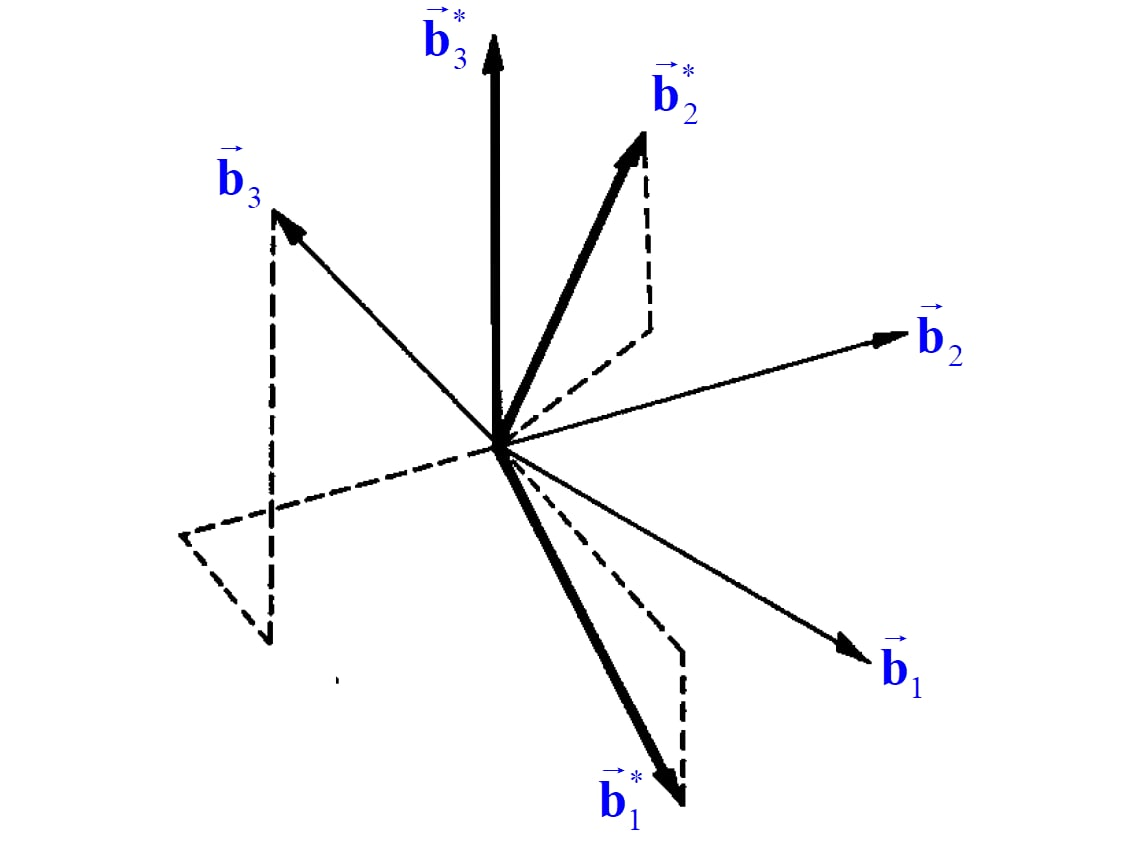
\includegraphics[scale=0.325]{Imagenes/Vectores_base_reciproco.jpeg}
    \caption{Conjuntos recíprocos de vectores base.}
\end{figure}
\end{frame}
\begin{frame}
\frametitle{Revisión importante}
Observemos lo siguiente: todos los vectores $\va{A}$, $\left\{ \va{b}_{1}, \va{b}_{2}, \va{b}_{3} \right\}$ y $\left\{ \va{b}_{1}^{*}, \va{b}_{2}^{*}, \va{b}_{3}^{*} \right\}$, están definidos en la base canónica de    $\mathbb{R}^{3}$ $(\vu{x}, \vu{y}, \vu{z})$.
\end{frame}
\begin{frame}
\frametitle{Misma representación de un vector}
Es decir, el vector $\va{A}$ puede tener \emph{diferentes representaciones}, sin embargo es el mismo vector.
\\
\bigskip
\pause
Esto nos lleva a concluir que una vez conocidas las componentes del vector $\va{A}$  en una base determinada, ese vector $\va{A}$ \textbf{queda determinado unívocamente}.
\end{frame}
\begin{frame}
\frametitle{Usando notación más compacta}
En ese sentido cada vector queda definido a través de sus componentes y puede emplearse un notación más compacta, denominada \emph{notación de índices}, en la cual un determinado vector se escribe como: $\va{A} = A_{i}$.
\end{frame}
\begin{frame}
\frametitle{Utilidad de la base recíproca}
Los vectores base no ortogonales son muy útiles en la física.
\\
\bigskip
\pause
Se ocupan en problemas relacionados con la propagación de ondas: electromagnéticas, elásticas, etc. así como en materiales que tengan una estructura periódica como los cristales.
\end{frame}
\begin{frame}
\frametitle{¿Qué es un cristal?}
Un cristal ideal es una estructura periódica, la cual es la misma cuando se le mira con respecto al punto interior del cristal elegido como origen, que cuando se le mira con respecto a todos los puntos.
\end{frame}
\begin{frame}
\frametitle{Posición dentro del cristal}
La posición dentro del cristal está dada por:
\pause
\begin{align*}
\vb{r} = \rho_{1} \, \vb{b}_{1} + \rho_{2} \, \vb{b}_{2} + \rho_{3} \, \vb{b}_{3}
\end{align*}
donde $\rho_{1}, \rho_{2}, \rho_{3}$ son números enteros.
\end{frame}
\begin{frame}
\frametitle{Los vectores en el cristal}
Los vectores $\vb{b}_{1}, \vb{b}_{2}, \vb{b}_{3}$ se denominan \emph{ejes del cristal o vectores primitivos de traslación} del cristal.
\\
\bigskip
\pause
El conjunto de puntos definido por los anteriores vectores de posición se llama \emph{red cristalina}. \pause Los vectores recíprocos $\vb{b}_{i}^{*}$ definen la \emph{red recíproca}.
\end{frame}


\section{Producto punto}
\frame{\tableofcontents[currentsection, hideothersubsections]}
\subsection{Ortogonalidad de las bases}

\begin{frame}
\frametitle{La base inicial y la recíproca}
Para poder referirnos al producto escalar, debemos responder una pregunta adicional: sobre la ortogonalidad de la base $\left\{ \va{b}_{1}, \va{b}_{2}, \va{b}_{3} \right\}$ y su base recíproca $\left\{ \va{b}_{1}^{*}, \va{b}_{2}^{*}, \va{b}_{3}^{*} \right\}$.
\end{frame}
\begin{frame}
\frametitle{Producto entre las bases}
Para este fin, usando la ec.(\ref{eq:ecuacion_01_05}) determinamos los productos:
\begin{align}
\begin{aligned}
\va{b}_{1}^{*} \cdot \va{b}_{2}^{*} \times \va{b}_{3}^{*} &= \dfrac{1}{\va{b}_{1} \cdot \va{b}_{2} \times \va{b}_{3}} \\[0.5em]
\va{b}_{i}^{*} \cdot \va{b}_{k} &= \delta_{i,k}
\end{aligned}
\label{eq:ecuacion_01_07}
\end{align}
donde $\delta_{i,k}$ es la delta de Kronecker.
\end{frame}
\begin{frame}
\frametitle{Evaluando el producto interno}
Usando la ec. (\ref{eq:ecuacion_01_07}) evaluamos el producto punto de dos vectores $\va{A}$ y $\va{B}$.
\\
\bigskip
\pause
Sean $\va{A}$ y $\va{B}$ dos vectores arbitrarios en las bases $\left\{ \va{b}_{1}, \va{b}_{2}, \va{b}_{3} \right\}$ y $\left\{ \va{b}_{1}^{*}, \va{b}_{2}^{*}, \va{b}_{3}^{*} \right\}$. 
\end{frame}
\begin{frame}
\frametitle{Evaluando el producto interno}
Mediante la relación entre ambas bases podemos calcular el producto punto de ambos vectores:
\pause
\begin{align}
\begin{aligned}
\va{A} &= \alpha_{1} \, \va{b}_{1}^{*} + \alpha_{2} \, \va{b}_{2}^{*} + \alpha_{3} \, \va{b}_{3}^{*} \\[0.5em] 
\va{B} &= \beta_{1}^{*} \, \va{b}_{1} + \beta_{2}^{*} \, \va{b}_{2} + \beta_{3}^{*} \, \va{b}_{3} \\[0.5em] 
\Rightarrow \hspace{0.4cm} \va{A} \cdot \va{B} &= \alpha_{1} \, \beta_{1}^{*} + \alpha_{2} \, \beta_{2}^{*} + \alpha_{3} \, \beta_{3}^{*} \\[0.5em]
&= \nsum_{l=1}^{3} \alpha_{l} \, \beta_{l}^{*}
\end{aligned}
\label{eq:ecuacion_01_08}
\end{align}
\end{frame}
\begin{frame}
\frametitle{Evaluando las operaciones}
Notemos que la ec. (\ref{eq:ecuacion_01_07}) permite evaluar las operaciones de la ec.(\ref{eq:ecuacion_01_08}) de manera sencilla a través de la relación $\va{b}_{l}^{*} \cdot \va{b}_{k} = \delta_{l, k}$.
\\
\bigskip
\pause
Sin embargo, la condición para ello es \emph{conocer ambas bases y las componentes de al menos uno de los vectores en la base recíproca}.
\end{frame}
\begin{frame}
\frametitle{Relacionando los vectores}
Veamos una forma diferente de escribir la ec. (\ref{eq:ecuacion_01_08}), \pause para ello relacionamos las componentes de los vectores en ambas bases por medio de una matriz $g$.
\end{frame}
\begin{frame}
\frametitle{Escribiendo un vector}
Sea $\va{A}$, un vector escrito en la base $\left\{ \va{b}_{1}, \va{b}_{2}, \va{b}_{3} \right\}$ y en la base recíproca$\left\{ \va{b}_{1}^{*}, \va{b}_{2}^{*}, \va{b}_{3}^{*} \right\}$:
\pause
\begin{align}
\va{A} = \underbrace{\nsum_{l=1}^{3} \alpha_{l} \, \va{b}_{l}^{*}}_\text{base recíproca} = \underbrace{\nsum_{k=1}^{3} \alpha_{k}^{*} \, \va{b}_{k}}_\text{base $\va{b}$}
\label{eq:ecuacion_01_09}
\end{align}
\pause
Veamos cómo es la relación entre los coeficientes.
\end{frame}
\begin{frame}
\frametitle{Vector como combinación lineal}
Ahora se escribe cada uno de los vectores $\va{b}_{l}^{*}$ como una combinación lineal de los vectores $\va{b}_{k}$:
\begin{align}
\va{b}_{l} = \nsum_{k=1}^{3} g_{l,k} \, \va{b}_{k}^{*}
\label{eq:ecuacion_01_10}
\end{align}
\pause
Al sustituir la ec.(\ref{eq:ecuacion_01_10}) en la ec. (\ref{eq:ecuacion_01_09}) se obtiene:
\end{frame}
\begin{frame}
\frametitle{Sustituyendo expresiones}
\begin{equation}
\begin{aligned}
\va{A} &= \nsum_{l=1}^{3} \alpha_{l}^{*} \, \va{b}_{l} = \\[0.25em] \pause
&= \nsum_{l=1}^{3} \alpha_{l}^{*} \bigg[ \nsum_{k=1}^{3} g_{l,k} \, \va{b}_{k}^{*} \bigg] = \\[0.25em] \pause
&= \nsum_{k=1}^{3} \bigg[ \nsum_{l=1}^{3} \alpha_{l}^{*} \, g_{l,k} \bigg] \, \va{b}_{k}^{*} = \\[0.25em] \pause
&= \nsum_{k=1}^{3} \alpha_{k} \, \va{b}_{k}^{*} =
\end{aligned}
\label{eq:ecuacion_01_11}
\end{equation}
\end{frame}
\begin{frame}
\frametitle{Sustituyendo expresiones}
Pero:
\pause
\begin{eqnarray*}
\alpha_{k} &=& \nsum_{l=1}^{3} \alpha_{l}^{*} \, g_{l,k} \\[0.5em] \pause
&\Rightarrow& \hspace{0.2cm} \alpha_{k}^{*} = \nsum_{l=1}^{3} \alpha_{l}\, g_{l,k}^{*}
\end{eqnarray*}
\pause
Esto nos da una relación entre los coeficientes de la base inicial y la base recíproca.
\end{frame}
\begin{frame}
\frametitle{Nuevos coeficientes}
Solo resta encontrar los coeficientes $g_{l,k}$:
\pause
\begin{equation}
\begin{aligned}
\va{b}_{l} = \nsum_{m=1}^{3} g_{m,l} \, \va{b}_{m}^{*}  \pause \hspace{0.2cm} &\Rightarrow \hspace{0.2cm} \va{b}_{l} \cdot \va{b}_{k} = \nsum_{m=1}^{3} g_{l,m} \, \va{b}_{m}^{*} \cdot \va{b}_{k} = \\[0.em] \pause
&= \nsum_{m=1}^{3} g_{l,m} \, \delta_{m,k} = \\[0.5em] \pause
&= g_{l,k} \pause \hspace{0.2cm} \Longleftrightarrow \hspace{0.2cm} \va{b}_{l} \cdot \va{b}_{k} = g_{l,k}
\end{aligned}
\label{eq:ecuacion_01_12}
\end{equation}
\pause
Los coeficientes $g_{l,k}$ tienen dos índices libres $l$, y $k$ y representan una matriz conocida como \textbf{tensor métrico}.
\end{frame}
\begin{frame}
\frametitle{Producto punto y el tensor métrico}
Finalmente veamos como puede escribirse el producto punto entre dos vectores en términos de las ec. (\ref{eq:ecuacion_01_08}) y la ec. (\ref{eq:ecuacion_01_12}):
\begin{equation}
\begin{aligned}
\va{A} \cdot \va{B} &= \underbrace{\nsum_{l=1}^{3} \alpha_{l} \, \beta_{l}^{*}}_\text{ec. (\ref{eq:ecuacion_01_08})} = \pause \underbrace{\nsum_{l=1}^{3} \alpha_{l} \, \nsum_{k=1}^{3} \beta_{k} \, g_{k,l}^{*}}_\text{ec. (\ref{eq:ecuacion_01_12})} = \\ \pause 
&= \nsum_{l=1}^{3} \nsum_{k=1}^{3} \alpha_{l} \, \beta_{k} \, g_{k,l}^{*} = \\[0.1em] \pause
&= g_{k,l}^{*} \, \alpha_{l} \, \beta_{k}
\end{aligned}
\label{eq:ecuacion_01_13}
\end{equation}
\end{frame}
\begin{frame}
\frametitle{Notación de la suma}
La última igualdad en la ec. (\ref{eq:ecuacion_01_13}):
\pause
\begin{align*}
= g_{k,l}^{*} \, \alpha_{l} \, \beta_{k}
\end{align*}
se sigue de la \emph{convención de Einstein}, es decir, cuando se tienen dos índices repetidos se implica una suma sobre dicho índice, así que está ya no debe anotarse.
\end{frame}
\begin{frame}
\frametitle{Generalización de las bases}
La generalización de la base $\left\{ \va{b}_{1}, \va{b}_{2}, \va{b}_{3} \right\}$ es conocida como \textbf{base covariante} \pause y la base recíproca $\left\{ \va{b}_{1}^{*}, \va{b}_{2}^{*}, \va{b}_{3}^{*} \right\}$ es conocida como \textbf{base contravariante}, esto se revisará más adelante junto con la interpretación geométrica de la misma.
\end{frame}
\end{document}